\section{Object 1}
\markright{Object 1}

The base and arch profile were sketched and extruded to form the stepped block, after which an angled gusset rib was added with a second boss-extrude. A fillet was applied to the top edge of the arch, and a cut-extrude removed material through the arch to form the through-hole.

\begin{figure}[H]
	\centering

	\begin{subfigure}[b]{0.32\textwidth}
		\centering
		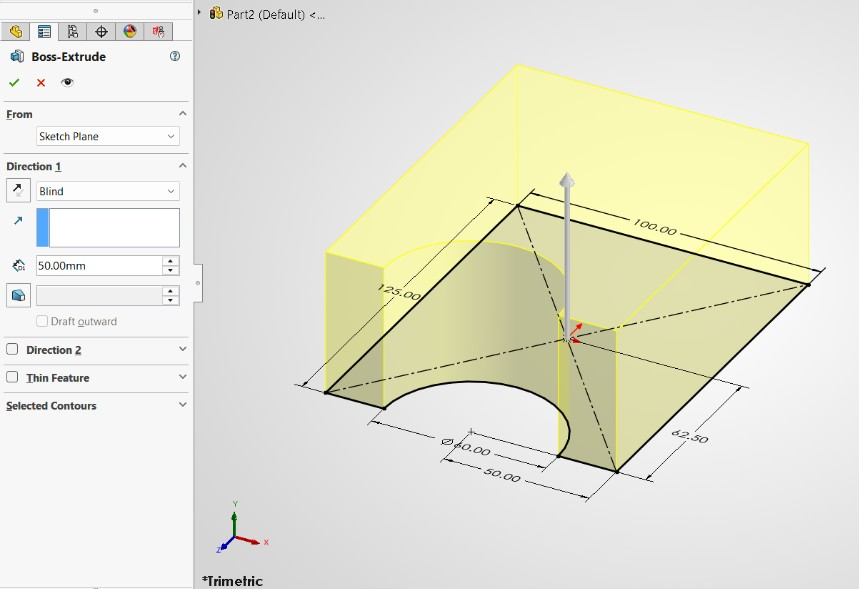
\includegraphics[width=\textwidth, keepaspectratio]{lab-02/assets/object-1/1.jpg}
		\caption{Boss-extrude preview of the base/arch profile}
	\end{subfigure}%
	\hfill
	\begin{subfigure}[b]{0.32\textwidth}
		\centering
		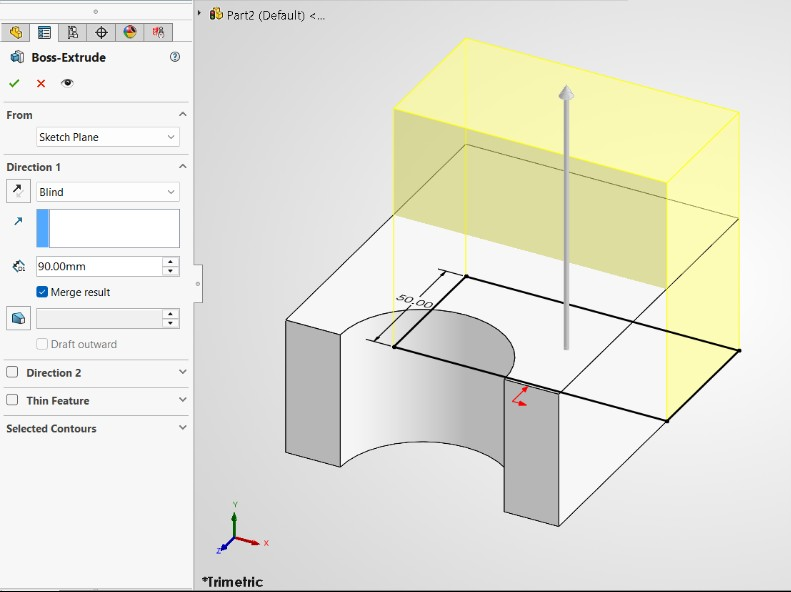
\includegraphics[width=\textwidth, keepaspectratio]{lab-02/assets/object-1/2.jpg}
		\caption{Extruding the base block}
	\end{subfigure}%
	\hfill
	\begin{subfigure}[b]{0.32\textwidth}
		\centering
		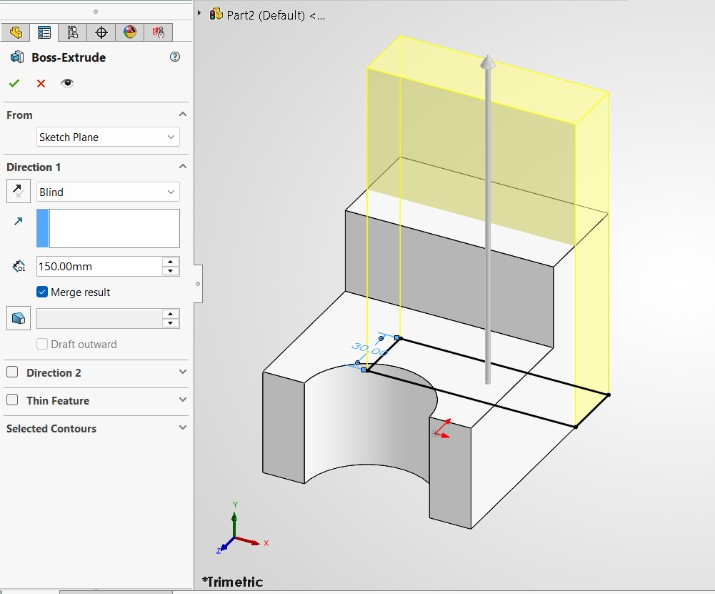
\includegraphics[width=\textwidth, keepaspectratio]{lab-02/assets/object-1/3.jpg}
		\caption{Boss-extrude dialog for the upper block}
	\end{subfigure}%
	\vspace{0.5em}
	\begin{subfigure}[b]{0.32\textwidth}
		\centering
		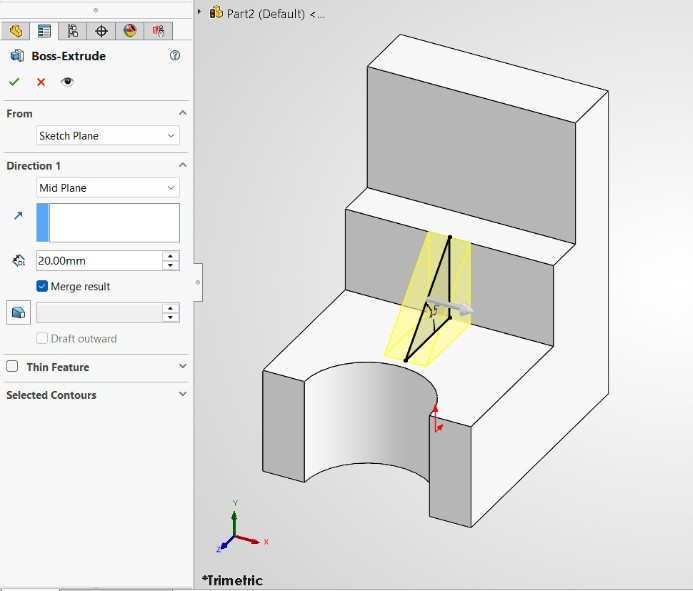
\includegraphics[width=\textwidth, keepaspectratio]{lab-02/assets/object-1/4.jpg}
		\caption{Extruding the angled support rib}
	\end{subfigure}%
	\hfill
	\begin{subfigure}[b]{0.32\textwidth}
		\centering
		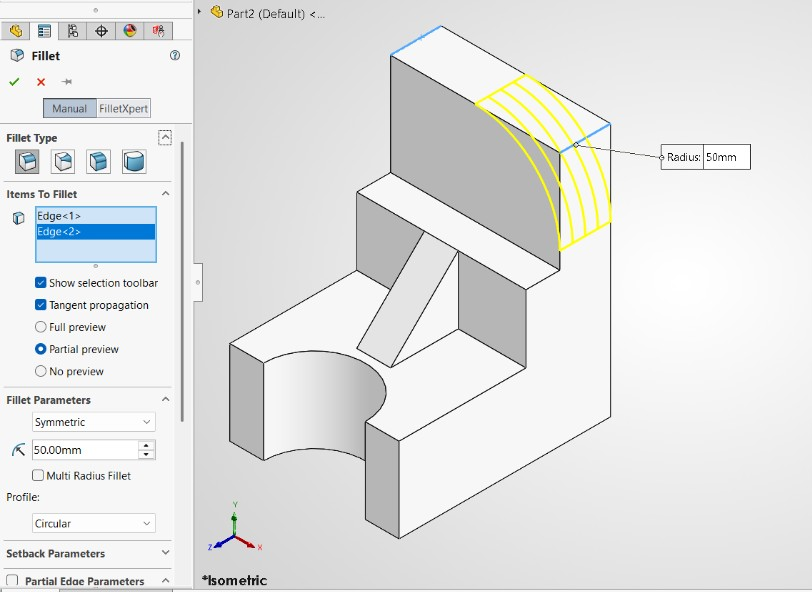
\includegraphics[width=\textwidth, keepaspectratio]{lab-02/assets/object-1/5.jpg}
		\caption{Applying a fillet to the arch edge}
	\end{subfigure}%
	\hfill
	\begin{subfigure}[b]{0.32\textwidth}
		\centering
		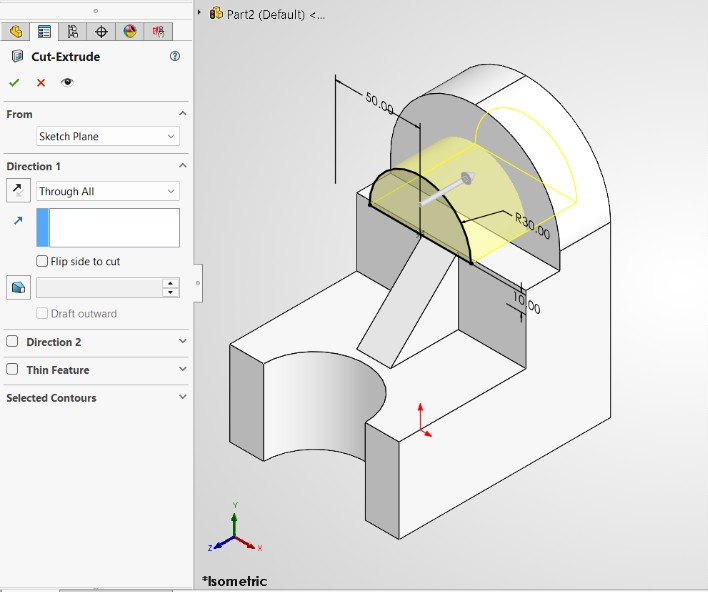
\includegraphics[width=\textwidth, keepaspectratio]{lab-02/assets/object-1/6.jpg}
		\caption{Cut-extrude forming the through-hole}
	\end{subfigure}%
	\vspace{0.5em}
	\begin{subfigure}[b]{\textwidth}
		\centering
		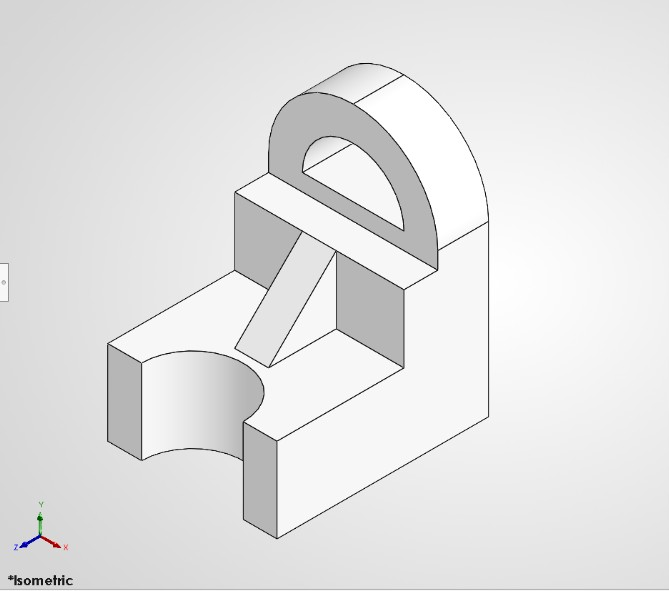
\includegraphics[width=\textwidth, keepaspectratio]{lab-02/assets/object-1/final.jpg}
		\caption{Final result}
	\end{subfigure}

	\caption{Snapshots while Designing Object 1 in Solidworks}
	\label{lab02_object_1}
\end{figure}
